\documentclass{report}
\usepackage{graphicx} % Required for inserting images
\usepackage[italian]{babel}
\usepackage{tikz}
\usepackage{hyperref}
\usepackage{amsmath}
\usepackage{xcolor}

\definecolor{darkgreen}{rgb}{0.0, 0.5, 0.0}


\title{Preferenze Privacy degli Utenti}
\date{Parte IV}

\begin{document}

\maketitle

\tableofcontents
\newpage

\chapter{Introduzione}
\subsubsection{Privacy dell'identità degli utenti}
Gli utenti preferiscono restare anonimi o comunque non condividere troppe informazioni quando
operano nel cloud.
Alcuni scenari:
\begin{itemize}
    \item \textbf{Tecniche di comunicazione anonima}
    \item \textbf{Privacy in location-based services} (protezione della location quando sensibile)
    \item \textbf{Attribute-based control access:} è un problema lato server, non ci si basa più su chi un tente sia (l'identità)
        ma sugli attributi che ha (certificati che l'utente presenta)
    \item \textbf{Supporto alle preferenze privacy degli utenti:} problema lato utente; \textit{se mi viene chiesto un documento d'identità, non è che do al server tutto il portafoglio}
\end{itemize}

\noindent Gli utenti potrebbero voler specificare le proprie scelte in termini di politiche del trattamento dei dati, quando:
\begin{itemize}
    \item condividono delle proprie risorse con server esterni (ad esempio i social media)
    \item vengono rilasciate informazioni nelle interazioni digitali (ad esempio lascio la carta di credito per accedere a un servizio)
\end{itemize}

$\rightarrow$ Due aspetti di \textbf{protezione:}
\begin{itemize}
    \item \textbf{rilascio diretto:} regola quando, a chi e perchè un utente rilascia informazioni (es. sto comprando qualcosa)
    \item \textbf{uso secondario:} regola l'uso e la profilazione dei dati da terze parti; anche questo deve essere sotto il controllo dell'utente
\end{itemize}

\section{Rilascio diretto}
La community di ricerca ha sviluppato diverse tecniche per regolare le interazioni
tra \textit{parti sconosciute}, definendo dei
meccanismi di \textbf{attribute-based access control}: consistono in una dipedenza dell'accesso rispetto alle proprietà che un utente ha.
Quello che gli utenti possono fare dipende dagli attributi che possiedono, verificati attraverso i \textbf{certificati}.

L'\textit{access control} non risponde più si o no, ma risponde con i requisiti che il richiedente deve soddisfare per avere l'accesso.
Non solo i server vanno protetti ma anche gli utenti, per questo vanno introdotte delle \textit{\textbf{forme di negoziazione}}.

\subsubsection{Esempio}

Se vogliamo cambiare filosofia, in un sistema aperto (non so chi è l'utente) se
voglio chiedere \textit{"tu soddisfi i requisiti per ottenere l'accesso?"}, 
nascono una serie di problematiche:
\begin{itemize}
    \item come specificare l'autorizzazione
    \item \textit{engine} per il controllo della politica
    \item anche la politica potrebbe essere confidenziale (\textit{non voglio dirti che faccio certi controlli})
    \item come chiedere le cose all'utente
    \item l'utente può avere delle controrichieste (\textit{hai la certificazione per chiedermi la carta di credito? la cripti?})
\end{itemize}

\noindent Questo dialogo deve terminare, deve essere \textbf{corretto} e \textbf{minimale}
nei termini delle informazioni rilasciate; tipicamente vengono usati linguaggi basati sul paradigma logico.

\newpage
\section{Controllo di accesso interattivo}
Il client è colui che richiede il servzio (utente), ha con sé:
\begin{itemize}
    \item \textbf{portfolio} (credenziali e proprietà)
    \item \textbf{stato}
    (stato di informazioni che vuole mantenere)
    \item \textbf{politica}
\end{itemize}

Lo stesso vale per il server, cioè colui che offre il servizio.

\subsection{Interazione senza condizioni da parte del client}
\begin{figure}[ht]
    \centering
    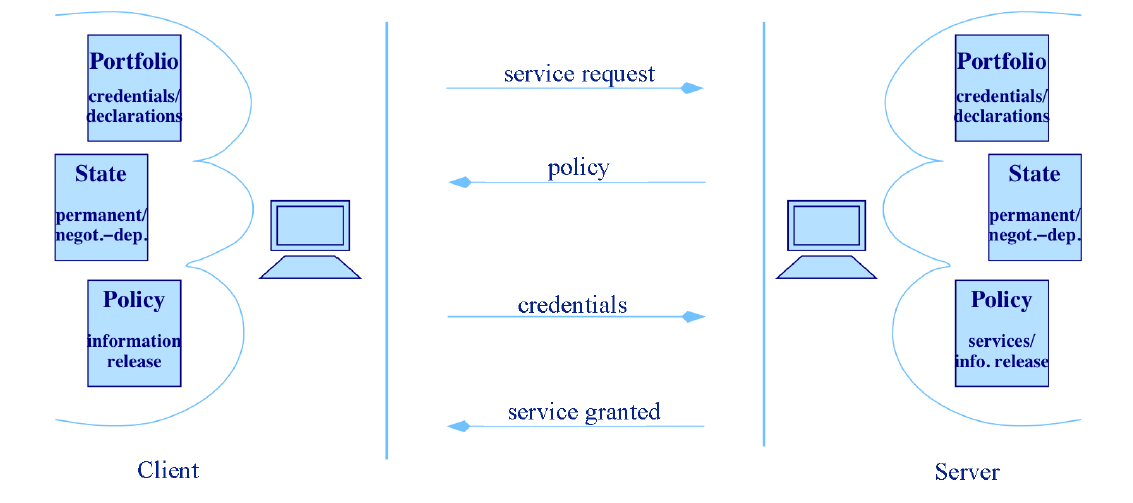
\includegraphics[width=1\linewidth]{images/interactive access control 1.png}
\end{figure}

\noindent La policy del server sta ad indicare ciò che il client deve dimostrare, tramite i certificati, per poter accedere al servzio.

\subsection{Negoziazione \textit{multi-step}}
\noindent In questo caso c'è una negoziazione tra client e server $ \rightarrow $ bisogna stabilire fiducia tra le due parti.

Il server per essere \textit{privacy-friendly} dovrebbe chiedere i dati tutti assieme.

\newpage
\subsection{Interazione a due step}
Per essere \textit{gentili} con l'utente viene fatta una distinzione tra i prerequsiti per l'accesso (necessari ma non sufficenti) e il requisito vero e proprio
con eventuale controrichiesta da parte dell'utente.

\begin{figure}[ht]
    \centering
    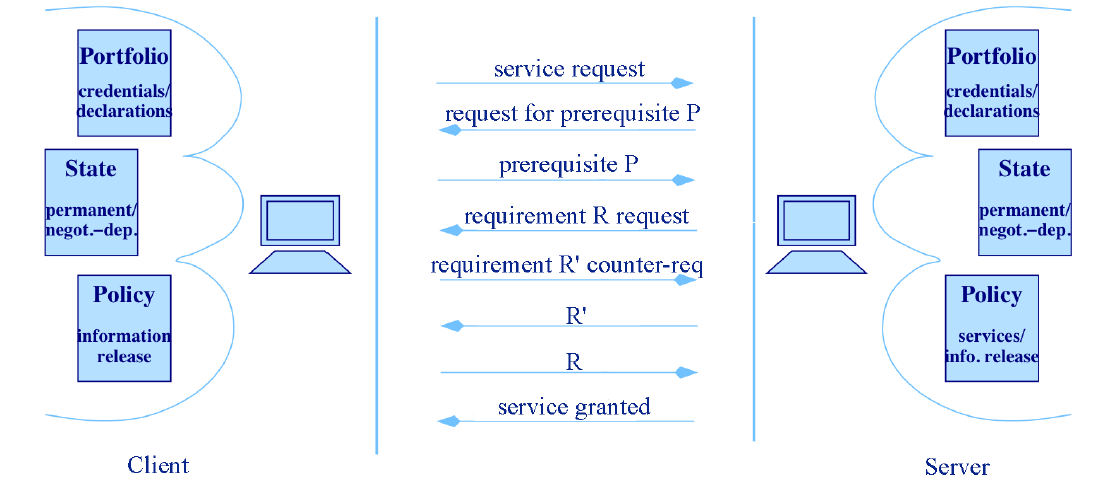
\includegraphics[width=1\linewidth]{images/interactive access control 2.png}
\end{figure}

\subsubsection{Esistenti/emegenti tecnologie di supporto a ABAC}
\begin{itemize}
    \item U-Prove/Idemix: fornisce avanzate tecnologie di gestione dei certificati (i certificati odierni ti permettono di estrapolare dal certificato solo
    l'informazione che voglio fornire all'altra parte, senza fornire tutto il certificato).
    \item XACML: standard di oggi per l'interoperabilità delle politiche di controllo degi accessi
\end{itemize}

\section{Preferenze degli utenti}

Le specifiche di controllo degli accessi non sempre si adattano bene con il problema lato utente:
\begin{itemize}
    \item \textcolor{darkgreen}{\textbf{+}} sono espressive, potenti e permettono all'utente di specificare se determinate informazioni possono o non possono essere rilasciate
    \item \textcolor{red}{\textbf{-}} non permettono agli uenti di esprimere che preferirebbero rilasciare determinate informazioni piuttosto che altre, nel contesto in cui ne sia data la possibilità
\end{itemize}

$\rightarrow$ È necessario fornire agli utenti strumenti per definire in modo efficace le preferenze sulla privacy riguardo al rilascio delle loro informazioni

\subsubsection{\textit{Desiderata}}
\begin{itemize}
    \item \textbf{Context-based preferences:} sono disposto a rilasciare un'informazione solo se mi trovo in un certo contesto (\textit{lascio la carta solo quando devo pagare})
    \item \textbf{Forbidden disclosures:} certe cose insieme non le rilascio
    \item \textbf{Associazioni sensibili:} associazioni che sono sensibili, perche sono \textit{quasi identifier} o perché non voglio che tu le veda
    \item \textbf{Limited disclosure:} \textit{se mi chiedi di essere maggiorenne, te lo dimostro ma non voglio dirti la mia età}
    \item \textbf{Instance-based preferences:} \textit{se la mia carta sta per scaedere, preferisco lasciarti quella}
    \item \textbf{History-based peferences:} magari ho già rilasciato qualcosa in passato
    \item \textbf{Proof-based preferences:} \textit{preferisco darti la prova che possiedo un passaporto invece che il passaporto stesso}
    \item \textbf{Non-linkability preferences:} \textit{preferisco lasciarti informzioni che, linkate con terze parti, mi identificano di meno}
\end{itemize}

\noindent Esistono diversi approcci per regolare la preferenza sulla privacy per gli utenti, 
che andiamo a vedere nei prossimi capitoli.

\chapter{Cost-sensitive Trust Negotiation}









\end{document}